\documentclass{beamer}

\usepackage[portuguese]{babel}
\usepackage[utf8]{inputenc}
\usepackage{minted}
\usepackage{graphicx}
\setbeamertemplate{footline}[frame number]

\title{Infraestrutura como Código (IaC) e Terraform}
\author[João Marcelo Uchôa de Alencar]{João Marcelo Uchôa de Alencar}
\institute{Universidade Federal do Ceará - Quixadá}

\begin{document}
   \begin{frame}
      \titlepage
   \end{frame}

   \begin{frame}
      \frametitle{Introdução}
      \begin{itemize}
      \item \textit{Infrastructure}\textit{ as }\textit{Code} (IaC):
      \begin{itemize}
      \item Escrever em código os recursos que compõe uma infraestrutura de TI.
      \item Automação.
      \end{itemize}
      \item Provisionamento: quais recursos criar.
      \item Configuração: definir as opções para cada recurso.
      \item Nuvens públicas e privadas oferecem operações através de APIs que permitem a plataformas IaC criar e configurar recursos. 
      \end{itemize}
   \end{frame}

   \begin{frame}
      \frametitle{Benefícios da IaC}
      \begin{itemize}
      \item Padronização da infraestrutura, já que podemos garantir que um ambiente de homologação é idêntico ao de produção se usarmos o mesmo código para gerar os dois.
      \item Possibilidade de controlar a evolução da infraestrutura em um sistema de gerenciamento de código.
      \item O próprio código pode ser integrado em um \textit{pipeline} CI/CD.
      \item Implantações que alteram a infraestrutura são mais rápidos e eficientes.
      \item Em geral, há redução de custo de infraestrutura pela possibilidade de análise do código que a instancia. 
      \end{itemize}
   \end{frame}

   \begin{frame}
      \frametitle{Linguagens IaC}
      \begin{itemize}
      \item Como a infraestrutura será descrita em código, precisamos de uma linguagem de programação.
      \item Três categorias:
      \begin{itemize}
      \item Linguagens de \textit{Scripts}.
      \item Linguagens de Declarativas.
      \item Linguagens de Programação Tradicionais.
      \end{itemize}
      \item Na prática, podem ser usadas em conjunto em um mesmo projeto.
      \end{itemize}
   \end{frame}

   \begin{frame}
      \frametitle{Linguagens de Scripts}
      \begin{itemize}
      \item Linguagens como \textit{bash} ou \textit{PowerShell}, que usam comandos para gerar sequências de ações para configurar infraestrutura. 
      \item No caso das nuvens, a maioria disponibiliza uma ferramenta em linha de comando (\textit{command}\textit{ }\textit{line}\textit{ interface }– CLI) que pode ser integrada em \textit{scripts.}
      \item Linguagens de \textit{scripts} tem poucas dependências e estão disponíveis na maioria dos sistemas operacionais.
      \item A desvantagem é que são de baixo nível, precisam de muitos comandos para realizar as atividades de criação e configuração de infraestrutura.
      \end{itemize}
   \end{frame}

   \begin{frame}[fragile]
      \frametitle{Linguagens de Scripts}
      \begin{itemize}
      \item Exemplo de criação de instância EC2 usando AWS CLI:   
      \end{itemize}
      \begin{minted}{bash}
aws ec2 run-instances \
  --image-id ami-0abcdef1234567890 \
  --count 1 \
  --instance-type t2.micro \
  --key-name MyKeyPair \
  --security-group-ids sg-903004f8 \
  --subnet-id subnet-6e7f829e
      \end{minted}
   \end{frame}

   \begin{frame}
      \frametitle{Linguagens Declarativas}
      \begin{itemize}
      \item O usuário não informa os comandos para criar os recursos, apenas declara quais as características do recurso a ser criado (estado desejado).
      \item Terraform, Ansible, Puppet, Chef, etc.
      \item A vantagem é que as especificações dos recursos que estão sendo criados são explícitas.
      \item A desvantagem é que o ambiente de execução é quem realizar as ações, então personalizações específicas exigem trechos em linguagens de \textit{scripts}.
      \end{itemize}
   \end{frame}

   \begin{frame}[fragile]
      \frametitle{Linguagens Declarativas}
      \begin{itemize}
      \item Exemplo de configuração Terraform (HCL):
      \end{itemize}
      \begin{minted}{terraform}
provider "aws" {
  region = "us-east-1"
}

resource "aws_instance" "example" {
  ami           = "ami-0abcdef1234567890"
  instance_type = "t2.micro"
  tags = {
    Name = "ExampleInstance"
  }
}
      \end{minted}
   \end{frame}

   \begin{frame}
      \frametitle{Linguagens Tradicionais}
      \begin{itemize}
      \item Linguagens já conhecidas pelos desenvolvedores, usadas para criar aplicações.
      \item TypeScript, Java, Python, Go, C\#, etc.
      \item A infraestrutura é descrita em programas que invocam bibliotecas e \textit{frameworks} para a criação dos recursos.
      \item A vantagem é que desenvolvedores podem auxiliar no processo de codificação de infraestrutura, pois já conhecem a linguagem. 
      \item Um possível desvantagem é que assim como linguagens de \textit{scripts}, o nível de abstração é baixo em relação às linguagens declarativas. 
      \end{itemize}
   \end{frame}

   \begin{frame}[fragile]
      \frametitle{Linguagens Tradicionais}
      \begin{itemize}
      \item Exemplo usando Python e boto3:
      \end{itemize}
      \begin{minted}{python}
import boto3

def create_ec2_instance():
    ec2 = boto3.resource('ec2', region_name='us-west-2')
    instance = ec2.create_instances(
        ImageId='ami-0abcdef1234567890',
        MinCount=1,
        MaxCount=1,
        InstanceType='t2.micro',
        KeyName='my-key-pair',
        SubnetId='subnet-6e7f829e',
        SecurityGroupIds=['sg-903004f8'],
    )
    print("Created instance", instance[0].id)

create_ec2_instance()
      \end{minted}
   \end{frame}

   \begin{frame}
      \frametitle{Metodologia IaC}
      \begin{itemize}
      \item Provisionamento de infraestrutura:
      \begin{itemize}
      \item É a criação dos recursos, sem configurá-los.
      \item Por exemplo, criar uma máquina virtual com SO e características de \textit{hardware} definidas, mas sem serviços como servidores \textit{web }ou banco de dados configurados.
      \end{itemize}
      \item Configuração de servidores e modelos:
      \begin{itemize}
      \item É a configuração do SO e dos serviços que o recurso irá hospedar.
      \item Por exemplo, dado o provisionamento prévio de uma VM, configurar o NGINX com WordPress.
      \item Modelos pré-existentes podem ser utilizados, também conhecidos como imagens. 
      \end{itemize}
      \end{itemize}
   \end{frame}

   \begin{frame}
      \frametitle{Metodologia IaC}
      \begin{itemize}
      \item Contêineres:
      \begin{itemize}
      \item Permite a uma mesma instância de VM hospedar aplicações de diferentes pilhas de \textit{software.}
      \item Por exemplo, uma instância pode hospedar uma aplicação Java ao mesmo tempo que executa código Python no Flask \textit{Framework}.
      \item O provisionamento pode criar uma instância padrão, sendo que a configuração é feita criando imagens de contêineres para cada aplicação.
      \end{itemize}
      \item Configuração e Implantação no Kubernetes:
      \begin{itemize}
      \item Permite a orquestração de contêineres.
      \item Um \textit{cluster} Kubernetes é a união de vários servidores.
      \item O sistema permite a distribuição de contêineres nos vários servidores, com alta flexibilidade e adaptabilidade.
      \end{itemize}
      \item Veremos mais detalhes sobre contêineres em um módulo posterior. 
      \end{itemize}
   \end{frame}

   \begin{frame}
      \frametitle{Conclusão}
      \begin{itemize}
      \item Tudo deve ser automatizado em código!
      \item O código deve estar no Git, de preferência, junto com o código da aplicação.
      \item Separar em uma hierarquia de diretórios de acordo com a infraestrutura.
      \item Integrar o código de infraestrutura ao \textit{pipeline} CI/CD.
      \item O código deve ser idempotente, ou seja, só criar os recursos que ainda não existem.
      \item O código deve ser modular. 
      \end{itemize}
   \end{frame}

   \begin{frame}
      \centering
      \Huge \textbf{Terraform}
   \end{frame}


   \begin{frame}
      \frametitle{Introdução}
      \begin{itemize}
      \item Instalar e configurar. 
      \item Escrever uma definição Terraform para implantar infraestrutura:
      \begin{itemize}
      \item \textit{Hashicorp}\textit{ }\textit{Configuration}\textit{ }\textit{Language}\textit{ }(HCL).
      \item Semelhante a sintaxe de arquivos JSON.
      \end{itemize}
      \item Entender as opções de linha de comando do Terraform.
      \item Boas práticas para organização dos arquivos Terraform.
      \end{itemize}
   \end{frame}

   \begin{frame}
      \frametitle{Instalação}
      \begin{itemize}
      \item Considerando Ubuntu como distribuição Linux.
      \item Vamos usar o gerenciador de pacotes \textit{apt}. 
      \item Instruções em. \url{https://developer.hashicorp.com/terraform/tutorials/aws-get-started/install-cli}.
      \end{itemize}
   \end{frame}

   \begin{frame}
      \frametitle{Etapas}
      \begin{itemize}
      \item Configurar o acesso à AWS.
      \item Configurar o provedor Terraform para AWS.
      \item Escrever código\textit{ }para criar infraestrutura na AWS:
      \begin{itemize}
      \item Separar em arquivos diferentes.
      \item Usar variáveis. 
      \end{itemize}
      \item Usar comandos Terraform para gerenciar a infraestrutura.
      \end{itemize}
   \end{frame}

   \begin{frame}[fragile]
      \frametitle{Configuração da AWS }
      \begin{itemize}
      \item Instalar a ferramenta de linha de comando da AWS usando uma das opções abaixo:
      \begin{itemize}
      \item 
      \footnotesize
      \begin{minted}{bash}
curl \
"https://awscli.amazonaws.com/awscli-exe-linux-x86\_64.zip" \
-o "awscliv2.zip"
unzip awscliv2.zip
sudo ./aws/install
sudo apt install awscli
      \end{minted}
      \normalsize
      \end{itemize}
      \item Configurar as variáveis de ambiente com as informações da \textit{AWS }\textit{Academy}:
      \begin{itemize}
      \item Copiar as informações de \textit{AWS }\textit{Details}\textit{/AWS CLI }no arquivo \textit{\~{}/.}\textit{aws}\textit{/}\textit{credentials}\textit{ }ou
      \item Configurar as variáveis de ambiente com os valores adequados:
      \begin{itemize}
      \item \$ export AWS\_ACCESS\_KEY\_ID="..."
      \item \$ export AWS\_SECRET\_ACCESS\_KEY="..."
      \item \$ export AWS\_SESSION\_TOKEN="..."
      \end{itemize}
      \end{itemize}
      \end{itemize}
   \end{frame}

   \begin{frame}[fragile]
      \frametitle{Exemplo de Arquivo Terraform}
      \begin{minted}{bash}
terraform {
  required_providers {
  aws = {
      source  = "hashicorp/aws"
      version = "~> 4.16"
    }
  }
  required_version = ">= 1.2.0"
}

provider "aws" {
   region = "us-east-1"
}
      \end{minted}
      \begin{itemize}
      \item Começamos definindo qual provedor vamos utilizar.
      \end{itemize}
      \begin{itemize}
      \item Configuramos o provedor AWS para usar a região indicada.
      \end{itemize}
   \end{frame}

   \begin{frame}[fragile]
      \frametitle{Exemplo de Arquivo Terraform}
      \footnotesize
      \begin{minted}{bash}
resource "aws_security_group" "devops" {
  name        = "devops"
  description = "Grupo de Seguranda da Disciplina DevOps"   
  tags = {
    Name = "devops"
  }
}

resource "aws_vpc_security_group_ingress_rule" "permitir_ssh_ipv4" {
  security_group_id = aws_security_group.devops.id
  cidr_ipv4         = "0.0.0.0/0"
  from_port         = 22
  ip_protocol       = "tcp"
  to_port           = 22
}
      \end{minted}
      \begin{itemize}
      \item Criamos um grupo de segurança (\textit{firewall}) para a disciplina.
      \end{itemize}
      \begin{itemize}
      \item Adicionamos uma regra para liberar o acesso ao SSH.
      \end{itemize}
   \end{frame}

   \begin{frame}[fragile]
      \frametitle{Exemplo de Arquivo Terraform}
      \begin{itemize}
      \item Criamos uma Máquina Virtual (Instância)
      \end{itemize}
      \begin{minted}{bash}
resource "aws_instance" "app_server" {
  ami             = "ami-0c7217cdde317cfec"
  instance_type   = "t2.micro"
  key_name        = "vockey"
  security_groups = ["devops"]
 
  tags = {
    Name = "InstanciaDevOps"
  }
}
      \end{minted}
      \begin{itemize}
      \item Informações específicas da região \textit{us-east-1}.
      \end{itemize}
      \begin{itemize}
      \item Grupo de Segurança. 
      \item Foi criado anteriormente.
      \end{itemize}
   \end{frame}

   \begin{frame}
      \frametitle{Comandos e Desenvolvimento Local}
   
      \begin{center}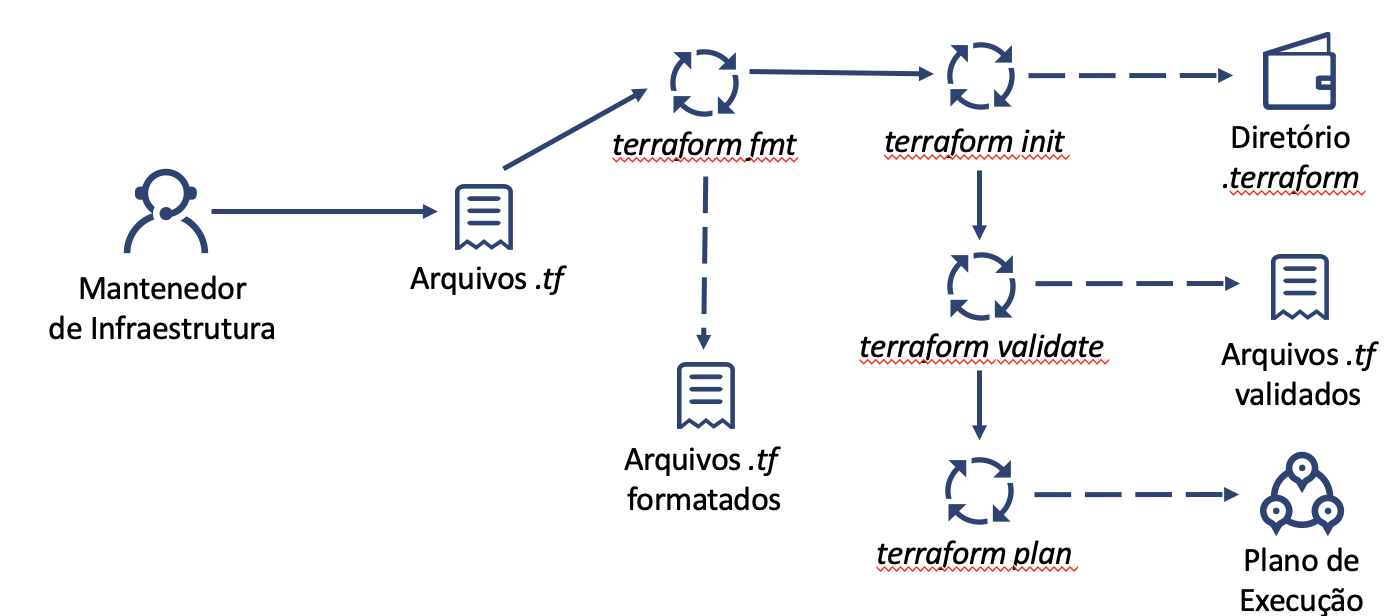
\includegraphics[width=1.0\textwidth,height=0.6\textheight,keepaspectratio]{images/comandoslocais.png}\end{center}
   \end{frame}

   \begin{frame}
      \frametitle{Integração Contínua}
   
      \begin{center}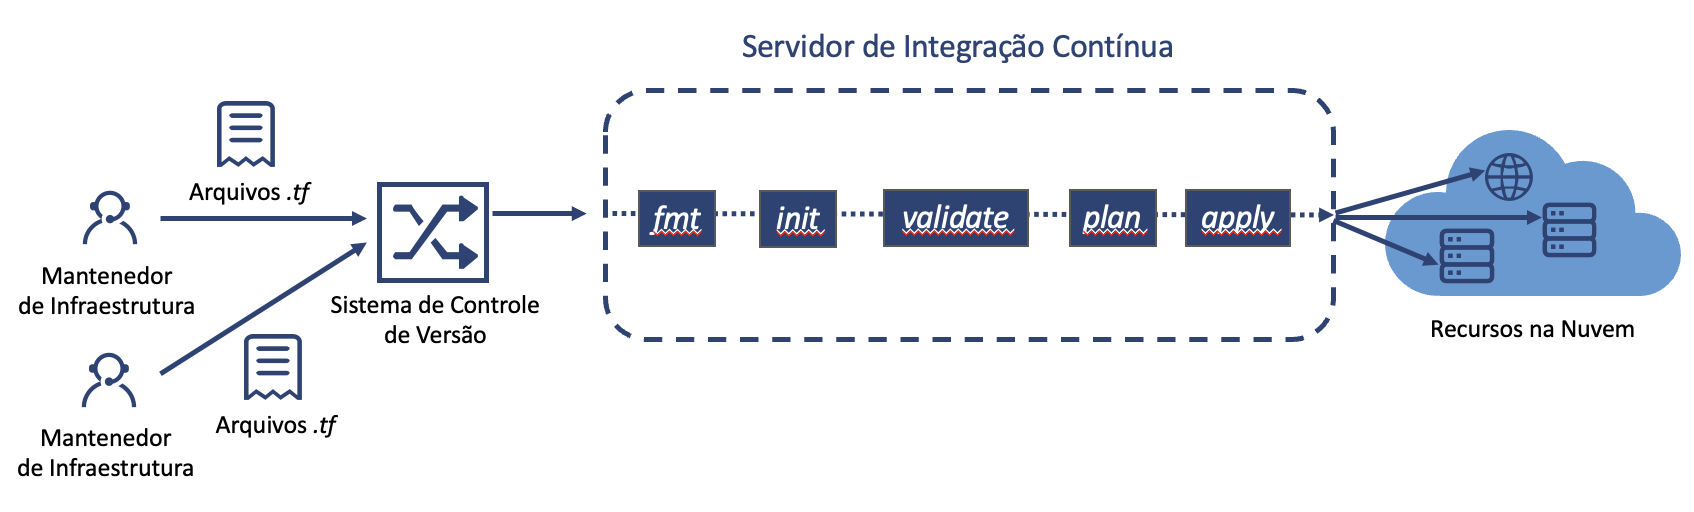
\includegraphics[width=1.0\textwidth,height=0.6\textheight,keepaspectratio]{images/integracaocontinua.png}\end{center}
   \end{frame}

   \begin{frame}
      \frametitle{Boas Práticas}
      \begin{itemize}
      \item No lugar um único arquivo (\textit{main.tf}), dividir em vários arquivos (\textit{main.tf}\textit{, }\textit{provider.tf}\textit{, }\textit{securitygroup.tf}\textit{, }\textit{etc}).
      \item Usar variáveis em um arquivo \textit{variables.tf} para aumentar a flexibilidade do código.
      \item Salvar o plano de ação em um arquivo:
      \begin{itemize}
      \item \textit{terraform}\textit{ }\textit{plan}\textit{ –out=}\textit{plano.tfplan}
      \item Semelhante a uma compilação, o arquivo \textit{plano.tfplan}\textit{ }pode ser aplicado a partir de outra estação de trabalho ou no servidor de Integração.
      \end{itemize}
      \end{itemize}
   \end{frame}

   \begin{frame}
      \frametitle{Boas Práticas}
      \begin{itemize}
      \item Guardar o arquivo de estado \textit{terraform.tfstate} na nuvem em um sistema de controle de versão:
      \begin{itemize}
      \item Esse arquivo contém o estado da infraestrutura. 
      \item Se várias pessoas trabalham na infraestrutura, é importante que todas acessem o estado corrente.
      \item Além do arquivo de estado \textit{terraform.tfstate}, o arquivo \textit{terraform.tfstate.lock.info} garante a sincronização
      \end{itemize}
      \item Precisamos adicionar um \textit{backend} de armazenamento.
      \item Na AWS, usamos um \textit{bucket} do S3.
      \end{itemize}
   \end{frame}

   \begin{frame}
      \frametitle{Boas Práticas}
      \begin{center}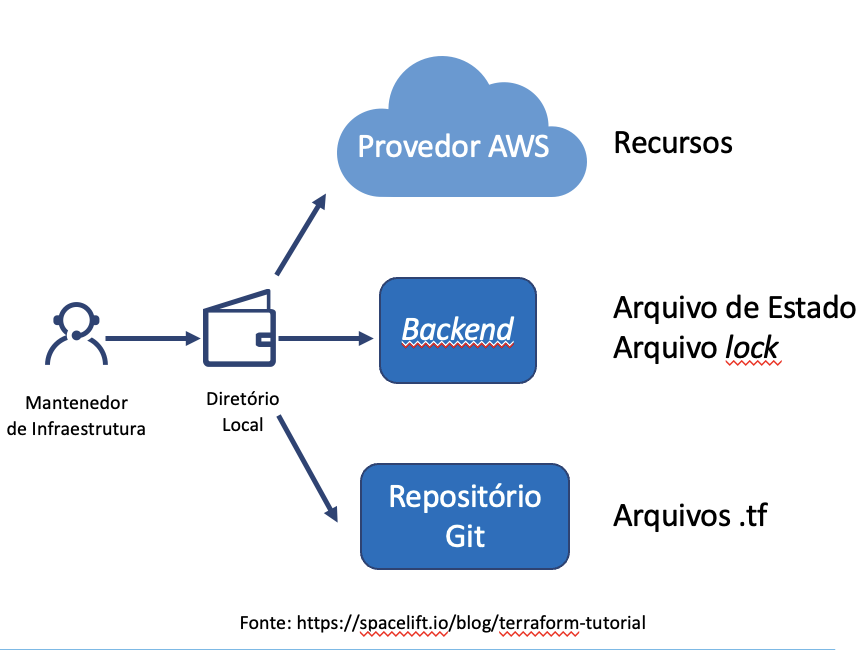
\includegraphics[width=1.0\textwidth,height=0.6\textheight,keepaspectratio]{images/boaspraticas.png}\end{center}
   \end{frame}

   \begin{frame}[fragile]
      \frametitle{Boas Práticas}
      \footnotesize 
      \begin{minted}{bash}
terraform {
 required_providers {
    aws = {
      source  = "hashicorp/aws"
      version = "~> 4.16"
    }
  }
  backend "s3" {
    bucket = "devops20240222"
    key    = "state"
  }
  required_version = ">= 1.2.0"
}

provider "aws" {
   region = "us-east-1"
}
      \end{minted}
      \begin{itemize}
      \item Criamos um \textit{bucket}\textit{ }(o nome precisa ser único):
      \begin{itemize}
      \item \$ aws s3 mb s3://devops2026013
      \end{itemize}
      \item Adicionamos o \textit{backend}\textit{ }no provedor.
      \item Podemos agora permitir várias equipes utilizando o mesmo arquivo. 
      \end{itemize}
   \end{frame}

   \begin{frame}
      \frametitle{Conclusão}
      \begin{itemize}
      \item Terraform permite usar uma linguagem declarativa para descrever recursos.
      \item É uma tecnologia para gerenciar infraestrutura nativa da nuvem.
      \item O uso de \textit{backend} na própria nuvem facilita o desenvolvimento da infraestrutura por equipes.
      \item Terraform pode ser usado tanto na linha de comando das estações de trabalho dos mantenedores quanto em execução em um servidor de Integração.
      \end{itemize}
   \end{frame}

\end{document}